% Drawing 57/01-1 -- folder 57, batch 01, archive page 15 (PDF page 16).
% Transcription: un diagramme à demi biffé, en partie écrit tête-bêche : des produits $P^1 \times P$, $P^0 \times_P P \rightrightarrows P_1 \to P$, des flèches verticales et une flèche courbe ; les termes ne se lisent pas assez pour être composés
% Kind: diagram of products (half struck). Method 2 (schematic redraw from the facsimile). Status: partial.
% Notes: Three rows, placed where he wrote them. Top: the struck stretch at the left of the row (a product ending in a heavy P^x) is not drawn; what is left unstruck is "x P", the double arrow and a heavy P. Middle: P^1 x P with a small cup-shaped sign under it, the downward arrow under the top P, and on the right the upward arrow to X. Bottom: P^0 x_P P, the double arrow, P_1 -> P. The curved arrow on the left runs from under the struck top row down to the bottom row. Labels at \small, as the transcription reads them (the letters on the card are a script P). Left out: the upside-down writing of the card at the top (two letters at the left and a line above), the scribbled blot under the right end of the bottom row. Still differs: the sign under P^1 x P (a cup, perhaps an inclusion or a short vertical arrow) is drawn as a cup; the exponents and subscripts are read after the transcription. Redrawn 2026-11-09 (issue 128): to check again.
% Coordinates: 1 unit = 1 mm = 1/100 of the crop width (bbox in page fractions: [0.1, 0.27, 0.46, 0.43]).
% Redrawn by Claude (claude-opus-5-5), issue #73, 2026-11-09; not checked by a human; not compiled (no TeX in the session).
% Rights: reproduces part of the work -- behind RENDER_TRANSCRIPTS, never published by itself.
\documentclass[tikz,border=3pt]{standalone}
\usepackage{amsmath,amssymb}
\usetikzlibrary{patterns,arrows.meta}
\tikzset{pencil/.style={black!45}, struck/.style={black!35}, mark/.style={circle,draw,inner sep=1.3pt}, pt/.style={circle,fill,inner sep=0.9pt}, opt/.style={circle,draw,fill=white,inner sep=1.1pt}}
\begin{document}
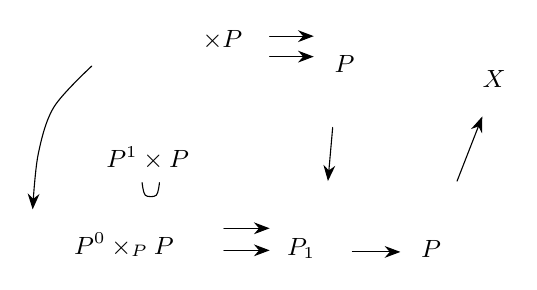
\begin{tikzpicture}[x=1mm,y=1mm,line cap=round,line join=round,font=\scriptsize]
\node[inner sep=1pt] at (57,-13.5) {\small $\times P$};
\draw[-{Stealth[length=2mm]}] (63,-13) -- (68.6,-13);
\draw[-{Stealth[length=2mm]}] (63,-15.6) -- (68.6,-15.6);
\node[inner sep=1pt] at (72.5,-16.5) {\small $P$};
\draw[-{Stealth[length=2mm]}] plot[smooth, tension=0.55] coordinates {(40.4,-16.8) (35.6,-22) (33.6,-28) (32.9,-35)};
\node[inner sep=1pt] at (47.5,-28.5) {\small $P^1\times P$};
\draw plot[smooth, tension=0.55] coordinates {(46.8,-31.6) (47.2,-33.2) (48.6,-33.2) (49,-31.6)};
\draw[-{Stealth[length=2mm]}] (71,-24.6) -- (70.4,-31.4);
\draw[-{Stealth[length=2mm]}] (86.8,-31.4) -- (90,-23.2);
\node[inner sep=1pt] at (91.5,-18.5) {\small $X$};
\node[inner sep=1pt] at (44.5,-39.5) {\small $P^0\times_P P$};
\draw[-{Stealth[length=2mm]}] (57.2,-37.4) -- (63,-37.4);
\draw[-{Stealth[length=2mm]}] (57.2,-40.2) -- (63,-40.2);
\node[inner sep=1pt] at (67,-40) {\small $P_1$};
\draw[-{Stealth[length=2mm]}] (73.5,-40.4) -- (79.6,-40.4);
\node[inner sep=1pt] at (83.5,-40) {\small $P$};
\end{tikzpicture}
\end{document}
